\documentclass{article}

\usepackage{pdfpages}
\usepackage{graphicx}

\usepackage{float}

\usepackage{adjustbox}
\usepackage{hyperref}

\graphicspath{ {./images/} }

\title{
    \vspace{-4.0cm}
    {\Huge Social Routing}\\[0.5cm]    
    \textsc{\Large Project and Seminar}\\[0.5cm]
    \textsc{\large Instituto Superior de Engenharia de Lisboa}\\[0.5cm]
}

\date{\today}
\author{   
    \begin{minipage}{0.4\textwidth}
        \begin{flushleft} \large
        \emph{Authors:}\\
        Baltasar Brito\\
        {\small email: baltasar.brito@gmail.com}\\
        {\small phone: 915953552}\\
        Bernardo Costa\\
        {\small email: bjmcosta97@gmail.com}\\
        {\small phone: 913897555}\\
        \end{flushleft}
    \end{minipage}
    ~
    \begin{minipage}{0.4\textwidth}
        \begin{flushright} \large
        \emph{Supervisor:} \\ 
        Pedro Félix\\
        {\small email: pedrofelix@cc.isel.ipl.pt}\\  
        \end{flushright}
    \end{minipage}\\[2cm]  
}

\begin{document}     
    
    \maketitle

    \newpage

    \tableofcontents

    \newpage

    
    
    \newpage
    \section{Report Structure}
    Each section of the report contains information about a component of the project's structure. 
    Each subsection represents a goal, established in the initial timeline, and contains information about it's completion and implementation. A link to the project's full documentation will also be included with every subsection.
    
    \section{System Structure}

    \begin{figure}[h]            
        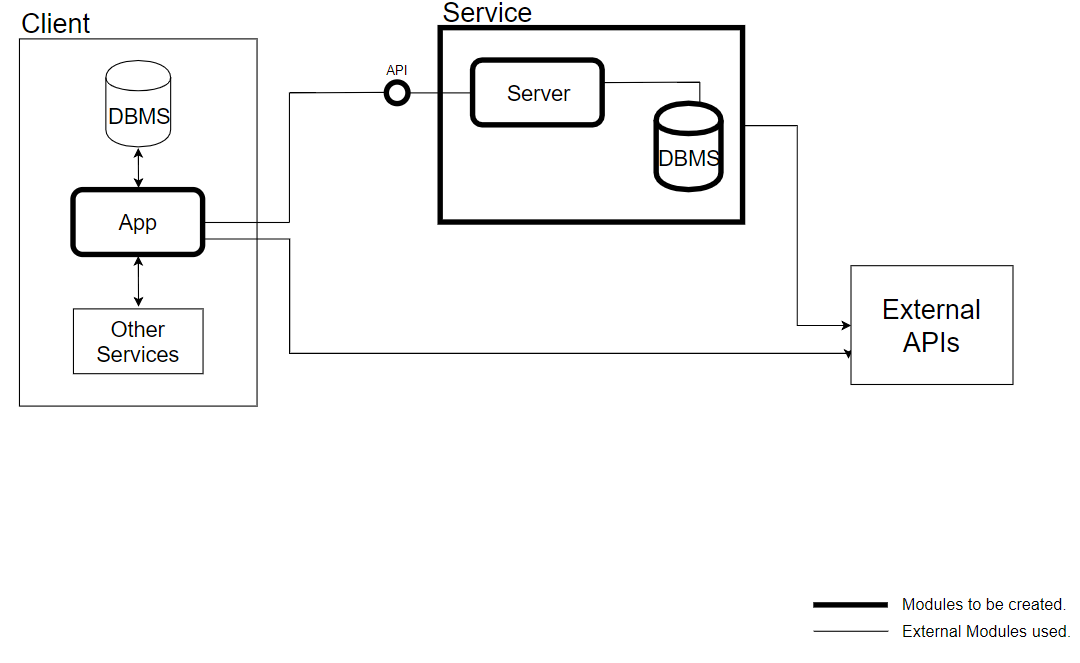
\includegraphics[width=\textwidth]{images/project-structure/system-structure.PNG}
        \caption{System structure.}
    \end{figure}  

    \newpage

    \section{Technologies}
    The technologies of the project are as follows:
    \begin{itemize}
        \item Client Application : Kotlin language, Gradle Build System. Using the frameworks: Todo
        \item Server : Kotlin language, Gradle Build System. Uses the framework JDBI, Spring, Todo
        \item Database Management System: PostgreSQL, uses SQL as language.
    \end{itemize}
    More details can be found \href{https://github.com/baltasarb/social-routing/wiki/1.-Choice-Of-Technologies}{here}.

    \newpage
    \section{Client Application}
   
    \newpage
    \section{Database Management System}
        \subsection*{Route Saving}
        Route saving is implemented in a for now incomplete version. Due to the nature of the project more features might be added, and as such a route characterization might change over time.
        Documentation link: TODO

        \subsection*{Add Remaining Necessary Objects}
        All the database objects are created and fully functional. 
        Documentation link: TODO
    \newpage
    \section{Server}    
        \subsection*{Communication with the Database Management System}
        The server communicates with the Database Management System through the \href{http://jdbi.org/}{jdbi API}, which is built on top of the jdbc driver.
        The communication is complete and is retrieving and inserting database objects correctly.
        Documentation \href{https://github.com/baltasarb/social-routing/wiki/3.-Communication-with-the-DBMS#jdbi}{link}.

        \subsection*{Infrastructure Design and Implementation}
        The server is designed following a repository pattern. All requests made to the API follow a pipeline:
        \begin{itemize}
            \item Controller: receives requests, exposed trough an API.
            \item Service : used by the controller to retrieve detailed information.
            \item Repository : Used by the services to retrieve or save information that exists only in the database.
        \end{itemize}
        Both the design and implementation are complete.
        Documentation \href{https://github.com/baltasarb/social-routing/wiki/4.-Server-design-and-implementation}{link}.

        \subsection*{Add All Functionalities Except Search}
        All basic functionalities are complete. A minimalistic version of a search is implemented to allow focus on other areas.
        Documentation link: TODO
    \newpage
    \section{Social Routing API}    
        \subsubsection*{Endpoint for Route Creation}
        The endpoint for route creation is complete.
        Documentation \href{https://github.com/baltasarb/social-routing/wiki/Social-Routing-API#create-route}{link}.
        \subsection*{Notes}
        The API was initially to be of focus later but is now close to complete, lacking only a more complex search functionality.
        Documentation for the full API can be found \href{https://github.com/baltasarb/social-routing/wiki/Social-Routing-API}{here}. 
        
    \section{Updated Timeline, Risks}

   
\end{document}
